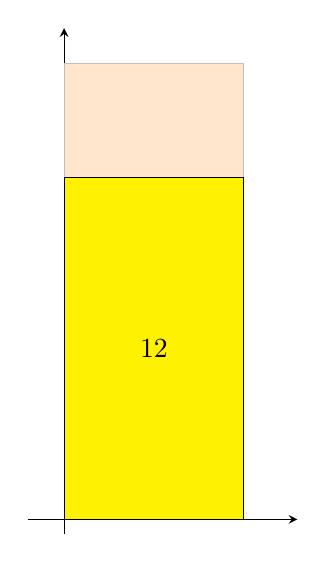
\begin{tikzpicture}
\begin{axis}[
		ticks=none,
        xmin =-.2,
        xmax = 1.3,
        ymax = 17.25,
        ymin = -0.5,
        width = 5cm,
        height = 8cm,
        axis x line = middle, axis y line = middle,
        every axis plot/.append style={ultra thick}]

	\draw [draw=lightgray, fill=orange, fill opacity=0.2] (0,0) rectangle node {$R$} (1, 16);
	\draw [fill = yellow] (0,0) rectangle node {12} (1,12);
	%\draw [fill = gray] (0,0) rectangle node {Streifen $S_0$} (10, 1) ;
	%\draw [fill = gray] (0,1) rectangle node {Streifen $S_1$} (10, 2) ;
	%\draw [fill = gray] (0,2) rectangle node {Streifen $S_2$} (10, 3) ;

	%\node[label={200:{$(0, 0)$}},circle,fill,inner sep=1.5pt] at (axis cs:0,0) {};
	%\node[label={200:{$(0, 12)$}},circle,fill,inner sep=1.5pt] at (axis cs:0,12) {};
	%\node[label={290:{$(N, B)$}},circle,fill,inner sep=1.5pt] at (axis cs:2,0) {};
	%\node[label={200:{$(0, E)$}},circle,fill,inner sep=1.5pt] at (axis cs:0,16) {};
	%\node[label={290:{$(N, E)$}},circle,fill,inner sep=1.5pt] at (axis cs:2,16) {};
	%\draw [fill = yellow] (0,7) rectangle node {} (5.26, 10) ;
\end{axis} 
\end{tikzpicture}
